\documentclass[aspectratio=169,11pt]{beamer}
\usepackage{presentation-theme}
\newcommand{\MaeAUC}{0.824}
\newcommand{\PromotedAUC}{0.814}
\newcommand{\InitialAUC}{0.834}
\newcommand{\LatestAUC}{0.814}
\newcommand{\MaccsDelta}{-0.020}
\newcommand{\RepeatCount}{2,659}
\newcommand{\RandomTanimoto}{0.095}
\newcommand{\MassTanimoto}{0.115}
\newcommand{\PermutationAUC}{0.497}

\hypersetup{pdftitle={Periodic teacher promotion: findings in five slides},pdfauthor={Wuhao}}
\newcommand{\bodytext}[4]{\node[anchor=north west,inner sep=0,align=left,text width=#3cm,font=\figurefont\fontsize{11}{14}\selectfont] at (#1,#2) {#4};}
\newcommand{\plotfigure}[1]{\node[anchor=north,inner sep=0] at (8,6.78) {\includegraphics[width=14.3cm,height=4.75cm,keepaspectratio]{../periodic_semantics/figures/#1_slide.pdf}};}
\begin{document}
\begin{frame}
\begin{tikzpicture}[remember picture,overlay,shift={(current page.south west)}]
\header{RESEARCH FINDINGS / 29 SEP 2026}{Promotion did not broadly improve chemical semantics}
\bodytext{1.0}{6.35}{13.7}{After \textbf{24 student-to-teacher promotions}, global chemical similarity and peak-dropout robustness improve. Chemical probes, local neighbors and repeat-spectrum retrieval worsen.}
\node[anchor=north west,inner sep=0,font=\brandmedium\fontsize{36}{40}\selectfont] at (1.0,4.3) {\InitialAUC\ \(\rightarrow\) \LatestAUC};
\bodytext{1.0}{2.9}{13.6}{Final-mean MACCS macro AUROC\\Initial teacher \(\rightarrow\) periodic student, step 1,209,000}
\takeaway{A useful embedding exists; automatic semantic improvement from promotion is not supported.}
\source{Fresh frozen-encoder audit: 231,104 spectra, 28,929 molecules. Chemical probes use 22,746 / 3,185 / 2,998 train / validation / test molecule centroids.}
\end{tikzpicture}
\end{frame}

\begin{frame}
\begin{tikzpicture}[remember picture,overlay,shift={(current page.south west)}]
\header{01 / CHEMICAL INFORMATION}{The initial teacher remains the stronger chemical readout}
\plotfigure{chemical_probes}
\takeaway{The comparison balances by molecule and chooses ridge penalties using validation data only.}
\source{Three exact states: initial JEPA teacher at 1,190,000; promoted teacher at periodic step 1,200,000; latest student at 1,209,000. Seven property targets and 15 functional groups.}
\end{tikzpicture}
\end{frame}

\begin{frame}
\begin{tikzpicture}[remember picture,overlay,shift={(current page.south west)}]
\header{02 / EMBEDDING GEOMETRY}{Check chemical neighbors without training a chemical head}
\plotfigure{geometry}
\takeaway{Native distances and train-fitted coordinate transformations are reported separately.}
\source{Morgan Tanimoto; test molecule queries against training molecule centroids. Partial rank correlation controls spectral similarity and precursor-mass difference. No supervised metric training.}
\end{tikzpicture}
\end{frame}

\begin{frame}
\begin{tikzpicture}[remember picture,overlay,shift={(current page.south west)}]
\header{03 / PRECISION}{The main differences survive paired molecule resampling}
\plotfigure{paired_uncertainty}
\takeaway{These intervals quantify held-out molecule sampling, not uncertainty across training runs.}
\source{95\% paired percentile intervals. 500 bootstrap resamples for AUROC; 2,000 for nearest-neighbor Tanimoto. Single pretraining seed; secondary measures are exploratory.}
\end{tikzpicture}
\end{frame}

\begin{frame}
\begin{tikzpicture}[remember picture,overlay,shift={(current page.south west)}]
\header{04 / INTERPRETATION}{Promotion is a training rule, not a semantic guarantee}
\bodytext{1.0}{6.5}{13.5}{\textbf{Plausible mechanism}\\Promotion can change which predictable signals the next generation learns.}
\bodytext{1.0}{4.95}{13.5}{\textbf{Measured result}\\Chemistry survives. Global ordering and dropout robustness improve; chemical readouts and local neighborhoods worsen.}
\bodytext{1.0}{3.25}{13.5}{\textbf{Decisive follow-up}\\Compare never-promoted and periodic teachers with matched student seeds, batches, masks, optimizer and training budget.}
\takeaway{Keep the hypothesis conditional; run the matched control before crediting or blaming promotion.}
\source{Full 21-slide report, speaker notes, experiment code, raw predictions and vector figure sources accompany this overview. No matched never-promoted experiment was run in this audit.}
\end{tikzpicture}
\end{frame}
\end{document}
